%---------------------------------------------------
% کلاس سند: article برای اسناد متنی، با اندازه کاغذ A4 و فونت پایه 16
\documentclass[a4paper,16pt]{article}

% بسته‌های ریاضی برای معادلات و نمادهای پیشرفته
\usepackage{amsmath, amssymb, amstext}

% بسته رنگ برای استفاده از رنگ در متن یا محیط‌ها
\usepackage{xcolor}

% بسته گرافیک برای درج تصاویر
\usepackage{graphicx}

% تنظیمات حاشیه صفحه
\usepackage{geometry}

% بسته لینک‌دهی (هایپرلینک‌ها)
\usepackage{hyperref}

% بسته صفحه‌آرایی برای تنظیم هدر و فوتر
\usepackage{fancyhdr}


% بسته xepersian برای پشتیبانی از زبان فارسی با XeLaTeX
\usepackage{xepersian}

% تعیین فونت فارسی (فایل فونت باید موجود باشد یا در سیستم نصب باشد)
\settextfont{B Nazanin}

% تنظیم اندازه حاشیه‌ها از هر طرف برابر با 1 اینچ
\geometry{margin=1in}

% تنظیم سبک fancy برای سربرگ و پاورقی
\pagestyle{fancy}

% سمت چپ هدر: مشخص‌کننده سری تمرین و نام درس
\lhead{تمرین سری سه درس فیزیک\lr{II }}

% وسط هدر: نام دانشکده
\chead{دانشکده فیزیک دانشگاه صنعتی خواجه نصیرالدین طوسی}

% سمت راست هدر: تاریخ روز به‌صورت خودکار
\rhead{\today}

% پایین صفحه: شماره صفحه
\cfoot{\thepage}

% شروع سند
\begin{document}
	
	% صفحه عنوان (بدون هدر و فوتر)
	\thispagestyle{empty}
	\begin{center}
		% لوگوی دانشگاه (باید فایل تصویر در مسیر پروژه باشد)
		
		
\includegraphics[width=0.5\textwidth]{../../../images/image-E_2/image-1.png} \\[10pt] 
		% عنوان سند
		\textbf{\LARGE عنوان:تمرین سری سه }\\[20pt]
		
		% نیم‌سال تحصیلی
		\textbf{\LARGE نیم‌سال تحصیلی:4032 }\\[10pt]
		
		% نام مدرس درس
		\textbf{\Large مدرس: ‫دكتر‬ ‫رضا‬ ‫افضل‬ ‫زاده‬}\\[10pt]
		
		% مبحث تمرین 
		\textbf{\Large ‫مبحث ‬‫تمرين‪:‬‬ ‫جريان‬ ‫الكتريكي‬ }\\[10pt]
		
		% مهلت تحویل تمرین
		\textbf{\Large ‫مهلت ‬‫تحويل‪:‬‬ ‫‪۳‬‬ ‫ارديبهشت‬ }
	\end{center}
	
	% صفحه جدید برای ادامه سند
	\newpage
	
	% ایجاد فهرست مطالب به‌صورت خودکار (براساس \section و \subsection و ...)
	\tableofcontents
	\newpage
	
	
	\section{سوال اول}

	جرياني كه در يك سيم با شعاع
	\[
	R = 3.40~\mathrm{mm}
	\]
	جريان دارد، چقدر است اگر چگالي جريان به صورت زير داده شده باشد:
	
	\begin{enumerate}
		\item[(الف)] 
		\[
		J(r) = a J_0, \quad 0 \le r \le R
		\]
		
		\item[(ب)] 
		\[
		J(r) = b J_0 \left(1 - \frac{r}{R}\right), \quad 0 \le r \le R
		\]
		
		كه در آن $r$ فاصله شعاعي از مركز سيم و
		\[
		J_0 = 5.50 \times 10^4~\mathrm{A/m^2}
		\]
		است.
		
		\item[(ج)] كدام يك از اين دو تابع، چگالي جريان را نزديك سطح سيم بيشينه مي كند؟
	\end{enumerate}
	
	\section{سوال دوم}
	يك سيم با مقاومت 
	\[
	R_0 = 6.0~\Omega
	\] 
	از قالبی عبور داده می‌شود، به طوری كه طول جديد آن سه برابر طول اوليه‌اش شود.  
	مقاومت سيم بلندتر را پيدا كنيد، با فرض اينكه مقاومت ويژه و چگالي ماده تغيير نكرده‌اند.
	\section{سوال سوم}
	يك دستگاه توان \(P = 18.0~\mathrm{W}\) و ولتاژ \(V = 9.00~\mathrm{V}\) دارد؛ مقدار بار عبوری در مدت \(t = 4.00~\mathrm{h}\) چقدر است؟
	
	\section{سوال چهارم}
	چگالي جريان در يك سيم يكنواخت بوده و بزرگی آن برابر با \(J = 2.0 \times 10^{10}~\mathrm{A/m^2}\) است. طول سيم \(L = 5.0~\mathrm{m}\) و چگالي الكترون‌های رسانش \(n = 8.49 \times 10^{28}~\mathrm{m^{-3}}\) می‌باشد. به طور میانگین، یک الكترون چه مدت زمان نیاز دارد تا طول سيم را طی كند؟
	\section{سوال پنجم}
در شكل زير، جريانی از يك مخروط ناقص دايره‌ای راست با مقاومت ويژه \(\rho = 731~\mathrm{m\cdot \Omega}\) عبور می‌کند. شعاع سمت چپ \(a = 2.00~\mathrm{mm}\)، شعاع سمت راست \(b = 2.30~\mathrm{mm}\) و طول \(L = 1.94~\mathrm{cm}\) است. فرض كنيد چگالي جريان در هر مقطع عمود بر طول يكنواخت باشد. مقاومت اين مخروط چقدر است؟
\begin{center}
	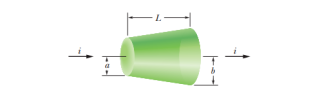
\includegraphics[width=0.5\textwidth]{../../../images/image-E_3/image-2.png} \\[10pt] 
\end{center}
	\section{سوال ششم}
	
يك ريسمان بسيار بلند با چگالي بار خطي \(\lambda\) روي محور يك دايره به شعاع \(r\) قرار داده شده است، به طوري كه انتهاي ريسمان در مركز دايره منطبق باشد. شار الكتريكي عبوري از سطح دايره را بيابيد.
	\section{سوال هفتم}
	بي‌نهايت بار نقطه‌اي به صورت يكي در ميان مثبت و منفي، با فاصله \(s\) از هم، روي يك خط راست چيده شده‌اند. انرژي برهم‌كنشي هر بار با ساير بارها را بر حسب \(s\) و بار \(q\) بيابيد.
	
	
	\textbf{موفق باشید.}
\end{document}
